

\documentclass{article}
\usepackage[utf8]{inputenc}
\usepackage{authblk}
\usepackage{setspace}
\usepackage[margin=0.6in]{geometry}
\usepackage{graphicx}
\graphicspath{ {./figures/} }
\usepackage{subcaption}
\usepackage[export]{adjustbox}
\usepackage{graphbox,graphicx}
\usepackage{floatrow}
\newfloatcommand{capbtabbox}{table}[][\FBwidth]
\usepackage{amsmath}
\usepackage{multirow}
\usepackage{float}


% \begin{figure}[H] se vuoi la posizione fissa
% \begin{figure}[h] altrimenti si sposta in automatico



%%%%%% Title %%%%%%
\title{Evaluating performance of TinyML on heterogeneous devices}

%%%%%% Authors %%%%%%
\author{Mattia Savoia}

%%%%%% Date %%%%%%
\date{}

\begin{document}

\maketitle

%%%%%% Main Text %%%%%%

\section{Introduction}
The advancements in machine learning (ML) opened a new opportunity to bring intelligence to the Internet-of-Things (IoT) nodes, such as microcontrollers. Conventional ML deployment has high memory and computes footprint obstruct their direct deployment on microcontrollers. 

TinyML can be defined as a subfield of Machine Learning which pursues enabling ML applications on devices that are cheap, as well as resource and power constrained. The objective of TinyML is to bring machine learning to the edge in an extreme way, where battery-powered, microcontroller-based embedded devices can perform ML tasks with real-time responsivity. 

The aim of this project is to evaluate the performance of different types of TinyML models on heterogeneous devices. The devices considered in this project are three microcontrollers (ESP32, ESP8266 and WEMOS D1 R32) and Machine Learning models have been performed on each of these devices. Exactly four Machine Learning models (Wine Classification, Handwritten Digits, Air Quality, Fashion Classification) were created, trained and saved. Each of these models was evaluated based on the prediction accuracy achieved.
At the end, the execution performance of these models on microcontrollers was evaluated by testing the execution time and memory footprint.

\section{Devices and Tools}
Three different devices were selected to compare their performance:
\begin{enumerate}
    \item \texttt{ESP32} is a series of low-cost, low-power system on a chip microcontrollers with integrated Wi-Fi and dual-mode Bluetooth. This board has 320 KB RAM, 1 MB Flash and a dual core processor. ESP32 has a clock speed of 240MHz.
    \item \texttt{ESP8266} is a low-cost Wi-Fi microchip. This board has 80 KB RAM, 1 MB Flash and a single core processor. ESP8266 has a clock speed of 80MHz.
    \item \texttt{WEMOS D1 R32} is ESP32 Based WiFi/Bluetooth Board in Arduino UNO form factor. So it has 320KB RAM, 1 MB Flash and a dual core processor. It has a clock speed of 240MHz. 
\end{enumerate}

To be able to evaluate the performance of ML models on microcontrollers, it is necessary to have several technologies available. In fact different tools have been used in this project:

\begin{itemize}
    \item \texttt{Python}: Python is an interpreted, object-oriented, high-level programming language with dynamic semantics. In this project it is used to create machine learning models.
    \item \texttt{C++}: C++ is a cross-platform language that can be used to create high-performance applications. In this project it is used to run the Machine Learning models on the microcontrollers.
    \item \texttt{TensorFlow}: TensorFlow is an open-source end-to-end platform for creating Machine Learning applications. It is a symbolic math library that uses dataflow and differentiable programming to perform various tasks focused on training and inference of deep neural networks. It allows developers to create machine learning applications using various tools, libraries, and community resources.
    \item \texttt{TensorFlow Lite}: TensorFlow Lite is a set of tools that enables on-device machine learning by helping developers run their models on mobile, embedded, and edge devices. This uses a custom memory allocator for execution latency and minimum load. It is also explaining the new file format supported Flat Buffers. TensorFlow Lite takes existing models and converts them into an optimized version within the sort of .tflite file.
    \item \texttt{PlatformIO}: PlatformIO is a cross-platform, cross-architecture, multiple framework, professional tool for embedded systems engineers and for software developers who write applications for embedded products. PlatformIO is a must-have tool for professional embedded systems engineers who develop solutions on more than one specific platform. In addition, by having a decentralized architecture, PlatformIO offers both new and existing developers a quick integration path for developing commercial-ready products, and reduces the overall time-to-market.
    \item \texttt{Project Inspector}: Project Inspector is a very useful PlatformIO tool which allows analyzing application memory usage (percentage of busy memory in RAM and in FLASH memory) and provides specific information about which memory section a variable or function is placed in or what file this symbol is located in. The report from Project Inspector a bit differs from the regular information reported after each build step. In this case, the differences can be explained by a different calculation method of memory consumption. Project Inspector also takes into account the memory section which was allocated for the stack and heap.
    \item \texttt{EloquentTinyML}: EloquentTinyML is an Arduino library to make TensorFlow Lite for microcontrollers neural networks more accessible and easy to use.
    \item \texttt{TinyMLgen}: TinyMLgen is a Python package to export TensorFlow Lite neural networks to C++ for microcontrollers.
\end{itemize} 


\section{Machine Learning Models}
Four different Machine Learning models have been created. To understand their reliability they were trained on a set of training data and tested on a set of test data, calculating the prediction accuracy through some metrics. Each of these models has different degrees of complexity in terms of ML algorithm and input size.

\subsection{Wine Classification Model (WC)}
The first model is \texttt{Wine Classification}. The Wine Dataset (from sklearn) was used. It contains 178 chemical analysis samples of wines belonging to 3 different classes (from 0 to 2). Each sample is described by 13 features. The data is the results of a chemical analysis of wines grown in the same region in Italy by three different cultivators. See Figure \ref{fig:1} for example.

\begin{figure}[H]
    \centering
    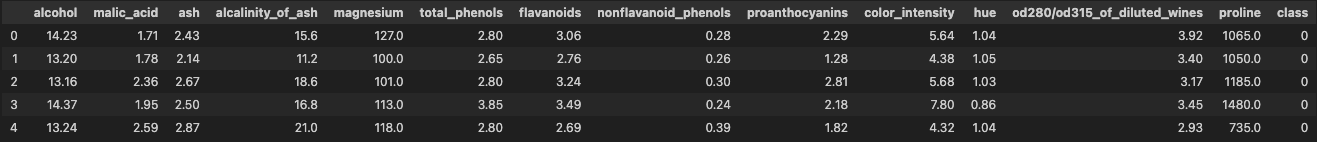
\includegraphics[width=0.95\textwidth]{WC-Dataset.png}
    \caption{Wine Dataset.}
    \label{fig:1}
\end{figure}

A fully connected network with 3 layers has been created. Once the model was trained on train data and tested on test data, the model was evaluated through the accuracy metric. \texttt{The accuracy result is about 77\%}. To perform a single prediction, it is necessary to pass a sample containing 13 features (alcohol, malic acid, ash, etc.) as input to the model. This will be able to predict the class of the sample.

\subsection{Handwritten Digits Model (HD)}
The second model is \texttt{Handwritten Digits}. The Digits Dataset (from sklearn) contains 1797 images of hand-written digits: 10 classes where each class refers to a digit (from 0 to 9). Each image is 8×8=64 pixels in size. See Figure \ref{fig:2} for example.

\begin{figure}[H]
    \centering
    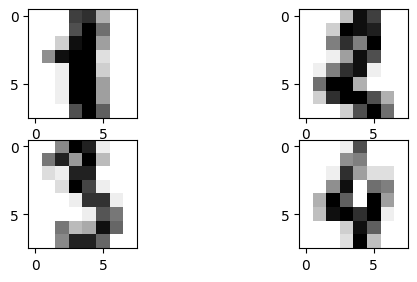
\includegraphics[width=0.3\textwidth]{HD-Dataset.png}
    \caption{Handwritten Digits Dataset.}
    \label{fig:2}
\end{figure}

A convolutional neural network with 5 layers has been created. Once the model was trained on train data and tested on test data, the model was evaluated through the accuracy metric. \texttt{The accuracy result is about 94\%}. The input of the model consists of an 8x8 pixel image where each feature has a value between 0 and 1. This will be able to predict the class it belongs to.

\subsection{Air Quality Model (AQ)}
The third model is \texttt{Air Quality}. The air-quality-india Dataset contains 1616 daily values of PM2.5 registered in India from 2017 to 2022. Among the different types of air pollution, PM2.5 kills the most people worldwide. It consists of particles smaller than approximately 2.5 microns – so small that billions of them can fit inside a red blood cell. See Figure \ref{fig:3} for example.

\begin{figure}[H]
    \centering
    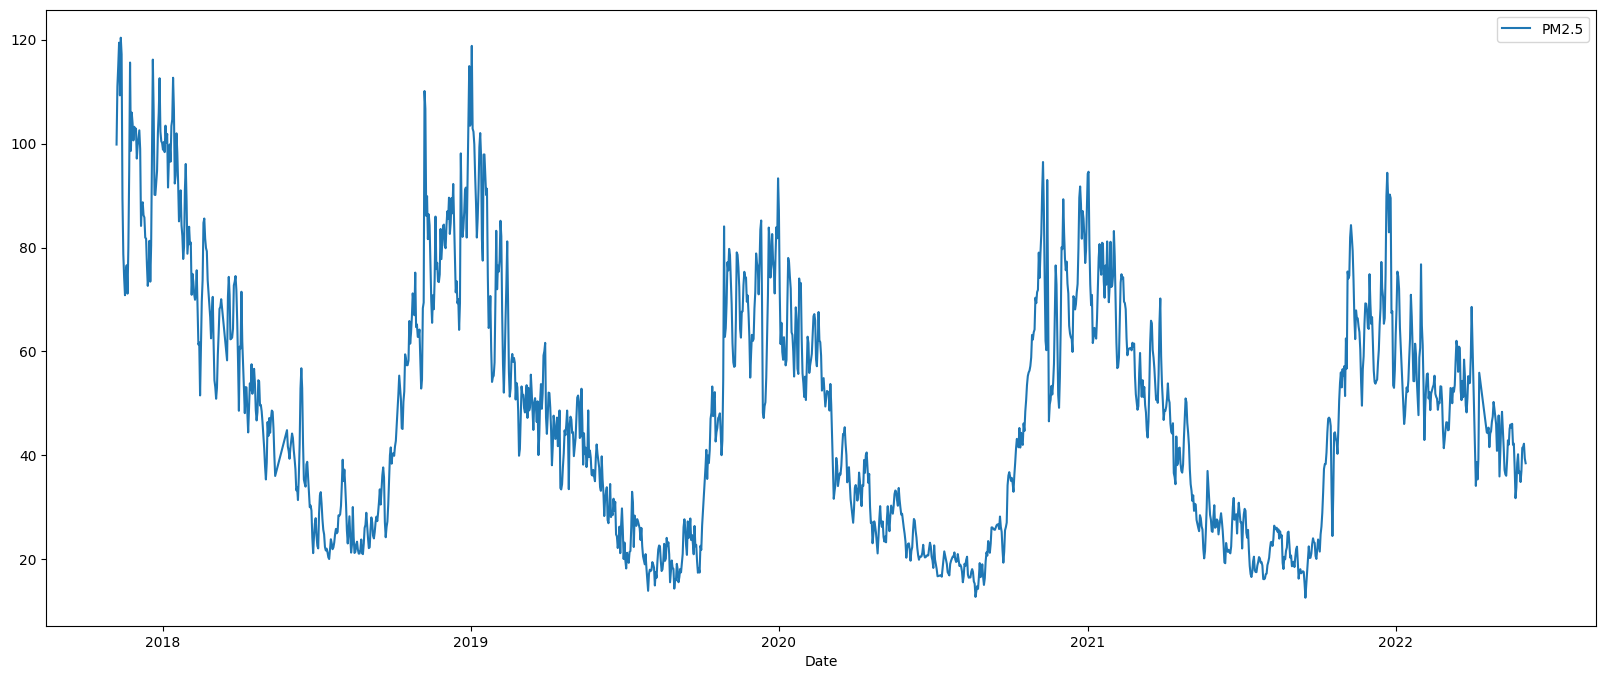
\includegraphics[width=0.9\textwidth]{AQ-Dataset.png}
    \caption{Air Quality Dataset.}
    \label{fig:3}
\end{figure}

A recurrent neural network with 2 layers has been created. After a phase of data preprocessing and once the model was trained on train data and tested on test data, the model was evaluated throught the MAE, MSE and MAPE metrics. \texttt{The MAE result is 3.43, the MSE is 26.0 and the MAPE is 8.34}. Given 5 samples as an input, the model is able to predict the future value of PM2.5. 

As you can see in Figure \ref{fig:4}, the model made predictions on the test set with a fairly high accuracy.

\begin{figure}[H]
    \centering
    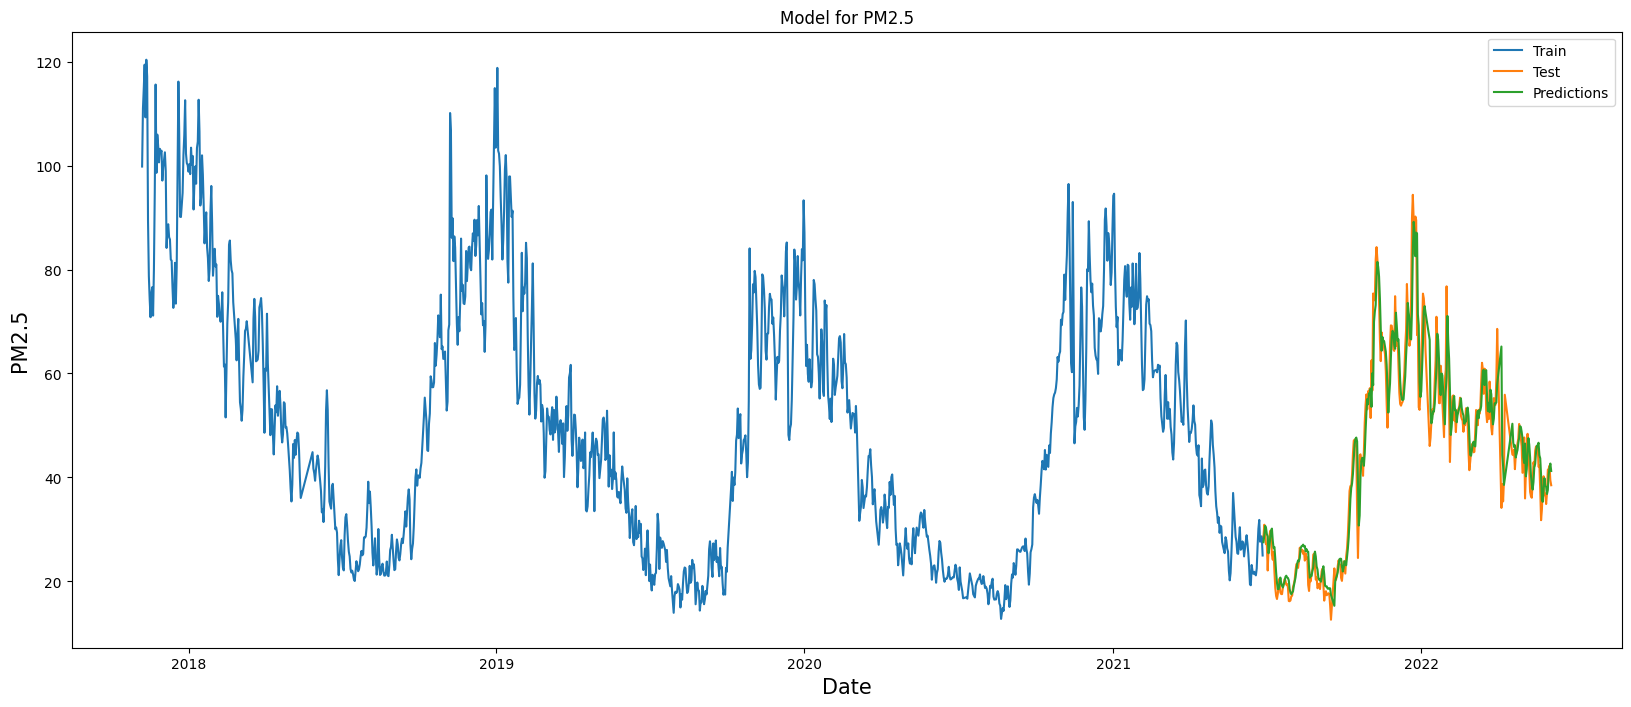
\includegraphics[width=0.9\textwidth]{AQ-Predictions.png}
    \caption{Air Quality Test Predictions.}
    \label{fig:4}
\end{figure}

\subsection{Fashion Classification Model (FC)}
The fourth model is \texttt{Fashion Classification}. Fashion Dataset (from MNIST) is a dataset of Zalando's article images consisting of 70000 samples (T-shirt, Sneaker, Pullover, etc.). Each image is 28 pixels in height and 28 pixels in width, for a total of 784 pixels, associated with a label from 10 classes (from 0 to 9). See Figure \ref{fig:5} for example. 

\begin{figure}[H]
    \centering
    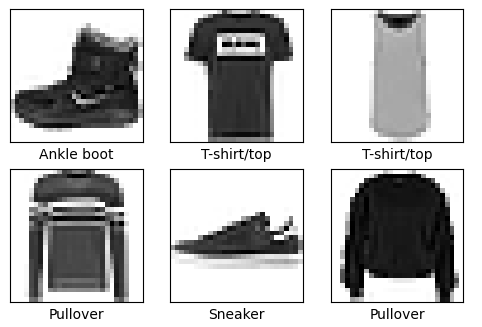
\includegraphics[width=0.6\textwidth]{FC-Dataset.png}
    \caption{Fashion Dataset.}
    \label{fig:5}
\end{figure}

A convolutional neural network with 4 layers has been created. Once the model was trained on train data and tested on test data, the model was evaluated through the accuracy metric. \texttt{The accuracy result is about 90\%}. The input of the model consists of an 28x28 pixel image where each feature has a value between 0 and 1. This will be able to predict the class it belongs to.

\subsection{Model conversion}
These four Machine Learning models were built through the TensorFlow library (written in Python code). It is therefore necessary to convert these models to C++ in order to run them on microcontrollers.

To do this the TinyMLgen library was used to port the Python code to C++ code. The models were saved in header files, then included in PlatformIO projects. In the main file of each PlatformIO project, the library EloquentTinyML was used to make TensorFlow Lite more easy to use. This technique was used only for the Wine Classification, Handwritten Classification and Fashion Classification models. Another technique was used for the Air Quality model because using a recurrent neural network (LSTM), EloquentTinyML does not work. In this case, the model had to be converted to TensorFlow Lite (.tflite) and the header file had to be created manually. To be able to use it, the header file was included in the main file of the project and TensorFlow Lite (for microcontrollers) was used directly instead of EloquentTinyML.

Once the models have been created and saved, it is then possible to use them on the microprocessors. In Table \ref{tab:1} you can see the file sizes of the saved ML models.

\begin{table}[H]
    \caption{Models sizes.}    
    \centering
    \begin{tabular}{ |c|c|c|c| } 
        \hline 
        {\bf WC} & {\bf HD} & {\bf AQ}  & {\bf FC} \\
        \hline 
        7,0 KB & 8,2 KB & 10,7 KB & 178,9 KB \\ 
        \hline
    \end{tabular}
    \label{tab:1}
\end{table}

\pagebreak 

\section{Time Analysis}
At this point we need to evaluate the prediction times of each model on all devices. A different PlatformIO project has been created for each model that runs on each device. In every single project, a function takes care of creating samples in a random way (simulating real data). These samples are passed as input to the model and then the prediction is calculated. In each project the function is called 100 times, thus collecting all prediction times. 

\subsection{WC predictions times}

\begin{minipage}{0.7\textwidth}
    \begin{figure}[H]
        \centering
        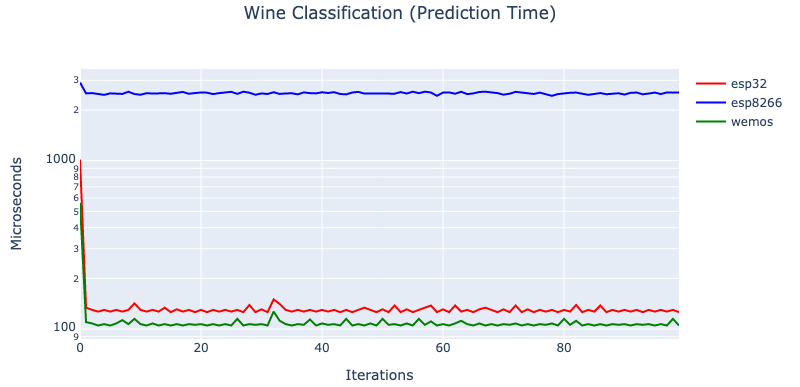
\includegraphics[scale=0.45]{WC-PredictionsTimes.png}
        \caption{WC predictions times.}
        \label{fig:6}
    \end{figure}
\end{minipage}
\hfill
\begin{minipage}{0.3\textwidth}
    \begin{table}[H]
        \caption{WC descriptive statistics.}    
        \centering
        \scalebox{0.7}{
            \begin{tabular}{ |c|c|c|c| } 
                \hline 
                & {\bf ESP32} & {\bf ESP8266} & {\bf WEMOS} \\
                \hline 
                {\bf mean} & 138,60 & 2517,57 & 111,95 \\ 
                \hline 
                {\bf std} & 88,82 & 50,41 & 45,38 \\ 
                \hline 
                {\bf min} & 126,00 & 2426,00 & 105,00 \\ 
                \hline 
                {\bf max} & 1017,00 & 2911,00 & 560,00 \\ 
                \hline
            \end{tabular}
        }
        \label{tab:2}
    \end{table}
\end{minipage}
\break

The Figure \ref{fig:6} shows the variations in the execution times of the three microcontrollers over 100 iterations to classify a Wine instance. The x-axis represents the iteration number, while the y-axis represents the execution time in microseconds. 

ESP8266 is slower than the other two boards. ESP32 and WEMOS have a trend that turns out to be quite similar, but the prediction values that WEMOS has, tell us that ESP32 is slower.

The first iteration is the one that takes longer than all the others. The TensorFlow runtime has components that initialize lazily, which can cause high latency for the first few predictions of a model after it has been loaded. This latency can be several orders of magnitude greater than that of a single prediction. For this reason the initial values can be considered as outliers.

The Table \ref{tab:2} contains descriptive statistics in relation to the prediction times of each microprocessor over 100 iterations. The values in the table are represented in microseconds. Based on the statistics, we can confirm that WEMOS is the faster board than the ESP32 and ESP8266 because it has a lower mean. Also regarding the standard deviation, WEMOS is the one that has the lowest value (however, it must be taken into consideration that ESP8266 has much larger values than WEMOS). 

More generally, the prediction times of the Wine Classification model on ESP8266 are about 18 times slower than ESP32 and WEMOS. Instead the difference between ESP32 and WEMOS is quite low, in fact WEMOS is on average 26 milliseconds faster than ESP32.

\subsection{HD predictions times}

\begin{minipage}{0.69\textwidth}
    \begin{figure}[H]
        \centering
        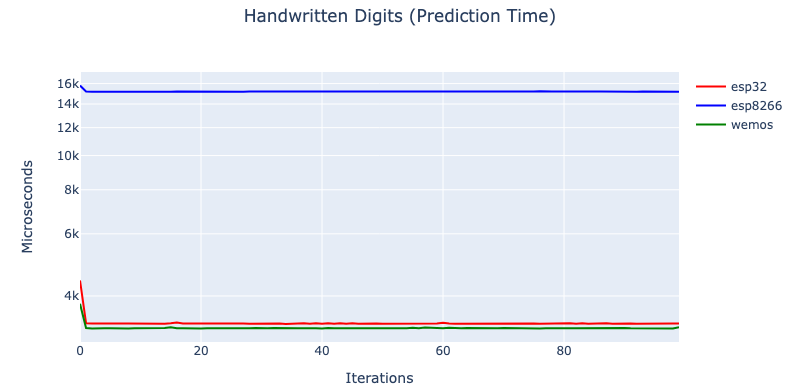
\includegraphics[scale=0.45]{HD-PredictionsTimes.png}
        \caption{HD predictions times.}
        \label{fig:7}
    \end{figure}
\end{minipage}
\hfill
\begin{minipage}{0.3\textwidth}
    \begin{table}[H]
        \caption{HD descriptive statistics.}    
        \centering
        \scalebox{0.7}{
            \begin{tabular}{ |c|c|c|c| } 
                \hline 
                & {\bf ESP32} & {\bf ESP8266} & {\bf WEMOS} \\
                \hline 
                {\bf mean} & 3351,67 & 15190,47 & 3246,18 \\ 
                \hline 
                {\bf std} & 108,51 & 62,45 & 56,03 \\ 
                \hline 
                {\bf min} & 3333,00 & 15159,00 & 3234,00 \\ 
                \hline 
                {\bf max} & 4425,00 & 15801,00 & 3799,00 \\ 
                \hline
            \end{tabular}
        }
        \label{tab:3}
    \end{table}
\end{minipage}
\break

The Figure \ref{fig:7} shows the performance of the three microcontrollers in terms of the time taken to predict the Handwritten Digits for 100 iterations. The x-axis represents the iteration number, while the y-axis represents the time in microseconds.

ESP8266 takes much longer to classify an instance than ESP32 and WEMOS which appear to be quite similar. Between ESP32 and WEMOS we can see that WEMOS is a bit faster, even if the difference doesn't seem big. The values in the graph appear to be constant, but this is because the values are represented on a very large scale on the y-axis.

As explained previously, the first iteration is the one that takes longer than all the others. These initial values can be considered as outliers.

The Table \ref{tab:3} contains descriptive statistics in relation to the execution times of each board over 100 iterations to classify an Handwritten Digits instance. The values in the table are represented in microseconds. From the descriptive statistics the mean of the prediction times of ESP8266 are highest, followed by ESP32 and WEMOS. The standard deviation in ESP32 is the highest, this means that there is more variability in measuring predictions (however, we always consider that ESP8266 has much larger values than WEMOS).

Generally, the prediction times of a Handwritten Digits instance turns out to be more than 4 times slower in ESP8266 than in ESP32 and WEMOS.

\subsection{AQ predictions times}

\begin{minipage}{0.69\textwidth}
    \begin{figure}[H]
        \centering
        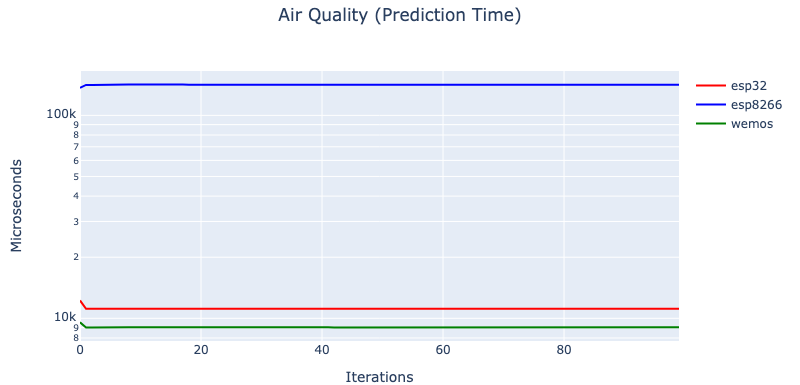
\includegraphics[scale=0.45]{AQ-PredictionsTimes.png}
        \caption{AQ predictions times.}
        \label{fig:8}
    \end{figure}
\end{minipage}
\hfill
\begin{minipage}{0.3\textwidth}
    \begin{table}[H]
        \caption{AQ descriptive statistics.}       
        \centering
        \scalebox{0.7}{
            \begin{tabular}{ |c|c|c|c| } 
                \hline 
                & {\bf ESP32} & {\bf ESP8266} & {\bf WEMOS} \\
                \hline 
                {\bf mean} & 11033,56 & 149737,25 & 8564.06 \\ 
                \hline 
                {\bf std} & 108,66 & 486.93 & 52.71 \\ 
                \hline 
                {\bf min} & 11010,00 & 144951,00 & 8550,00 \\ 
                \hline 
                {\bf max} & 12108,00 & 149833,00 & 9084,00 \\ 
                \hline
            \end{tabular}
        }
        \label{tab:4}
    \end{table}
\end{minipage}
\break

The Figure \ref{fig:8} shows the execution times of the three boards over 100 iterations to predict Air Quality. The x-axis represents the iteration number, while the y-axis represents the prediction time in microseconds. 

Also in this case ESP8266 turns out to be much slower than the other two microcontrollers. As in the previous cases also here the prediction times of WEMOS are faster than ESP32. The values in the graph appear to be constant, but this is because the values are represented on a very large scale on the y-axis.

The Table \ref{tab:4} contains descriptive statistics in relation to the execution times of each microcontrollers over 100 iterations to predict Air Quality. The values in the table are represented in microseconds. The descriptive statistics confirm that the ESP8266 turns out to be the slowest microncontroller compared to the other two, having a higher mean prediction time. The standard deviation of ESP8266 is the highest one, in fact the variability of the prediction is quite high, while WEMOS has a relatively low standard deviation (however, we always consider that ESP8266 has much larger values than WEMOS). 

More generally, the prediction times of the Air Quality model on ESP8266 are more than 13 times slower than ESP32 and WEMOS.

\subsection{FC predictions times}

\begin{minipage}{0.69\textwidth}
    \begin{figure}[H]
        \centering
        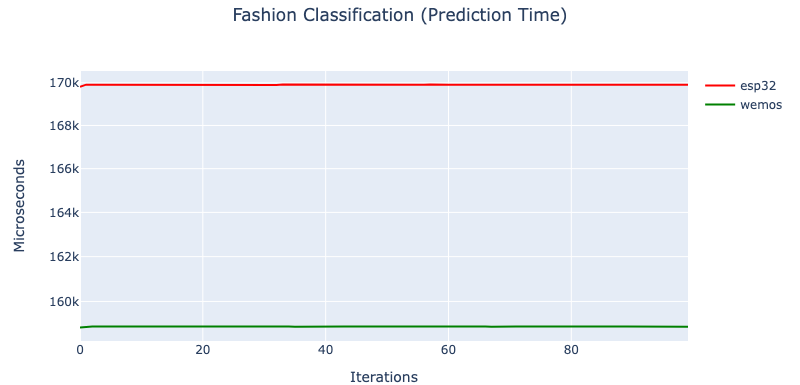
\includegraphics[scale=0.45]{FC-PredictionsTimes.png}
        \caption{AQ predictions times.}
        \label{fig:9}
    \end{figure}
\end{minipage}
\hfill
\begin{minipage}{0.3\textwidth}
    \begin{table}[H]
        \caption{FC descriptive statistics.}          
        \centering
        \scalebox{0.7}{
            \begin{tabular}{ |c|c|c|c| } 
                \hline 
                & {\bf ESP32} & {\bf WEMOS} \\
                \hline 
                {\bf mean} & 169908,93 & 158892,71 \\ 
                \hline 
                {\bf std} & 108,66 & 52.71 \\ 
                \hline 
                {\bf min} & 11010,00 & 8550,00 \\ 
                \hline 
                {\bf max} & 12108,00 & 9084,00 \\ 
                \hline
            \end{tabular}
        }
        \label{tab:5}
    \end{table}
\end{minipage}
\break

The Figure \ref{fig:9} shows the performance of the microcontrollers in terms of the time taken to predict the Fashion images for 100 iterations. The x-axis represents the iteration number, while the y-axis represents the time in microseconds. The ESP8266 board was unable to run this model due to insufficient RAM space. Therefore, the performance of this model on the ESP8266 board will not be considered. 

Prediction time of the ESP32 turns out to be a bit slower than WEMOS. The values in the graph appear to be constant, but this is because the values are represented on a very large scale on the y-axis.

The Table \ref{tab:5} contains descriptive statistics in relation to the execution times of the two boards over 100 iterations to classify a Fashion image. The values in the table are represented in microseconds. These stats confirm that WEMOS is faster than ESP32. The standard deviation of ESP32 is higher than WEMOS. 

In general the difference in prediction times between ESP32 and WEMOS is not very high.

\section{Memory Footprint Analysis}

To analyze the occupied memory usage on each device running the same model, some information was obtained from the PlatformIO Project Inspector. This information is data about the device's memory, so RAM and FLASH have been analyzed.

The microcontroller has 2 types of memory:
\begin{itemize}
    \item \texttt{RAM (Random-Access Memory)}: is a random access memory, and refers to the temporary storage component. It is a volatile memory that stores variables during the execution of a program and offers fast read access times.
    \item \texttt{FLASH memory}: is a non-volatile memory chip used for storage. It is used to store the program.
\end{itemize}

Using the EloquentTinyML or TensorflowLite library in each PlatformIO project created, it was necessary to set a Tensor Arena value. This value is used to allocate memory for the model tensors and this affects memory usage. In fact, the smallest possible value was selected for each type of model. Table \ref{tab:6} shows the Tensor Arena sizes used for each Machine Learning model. 

\begin{table}[H]
    \caption{Models Tensor Arena Sizes.}    
    \centering
    \begin{tabular}{ |c|c|c|c|c| } 
        \hline 
        & {\bf WC} & {\bf HD} & {\bf AQ} & {\bf FC} \\
        \hline 
        {\bf Tensor Arena (Bytes)} & 2*1024 & 4*1024 & 6*1024 & 90*1024 \\ 
        \hline
    \end{tabular}
    \label{tab:6}
\end{table}

\subsection{WC Memory Footprint}

\begin{figure}[H]
    \centering
    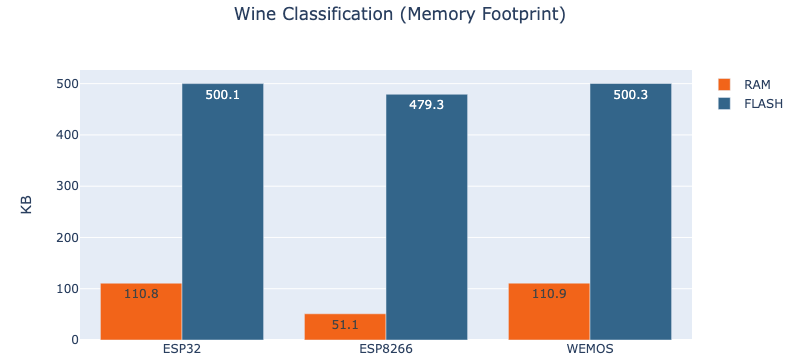
\includegraphics[width=0.6\textwidth]{WC-Mem-KB.png}
    \caption{WC Memory Footprint KB.}
    \label{fig:10}
\end{figure}

Figure \ref{fig:10} shows the memory usage (in KB) of the microcontrollers in relation to the Wine model. The x-axis represents the type of microcontroller, while the y-axis represents the amount of memory in KB. The ESP32 board has the same memory consumption as the WEMOS board. As for the ESP8266 in terms of FLASH it is quite similar (slightly inferior) to ESP32 and WEMOS, while RAM has a lower value in terms of KB.

\begin{figure}[H]
    \centering
    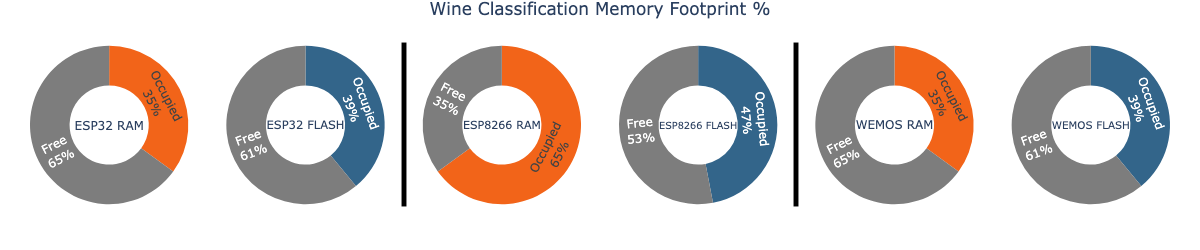
\includegraphics[width=1.0\textwidth]{WC-Mem-perc.png}
    \caption{WC Memory Footprint Percentages.}
    \label{fig:11}
\end{figure}

Figure \ref{fig:11} shows the memory usage as a percentage in relation to the Wine model of the three boards. ESP32 and WEMOS have the same percentage of occupied memory because the available memory is the same. ESP8266 has a higher percentage of occupied memory than the other two microcontrollers (the percentage of occupied RAM is quite high).

\subsection{HD Memory Footprint}

\begin{figure}[H]
    \centering
    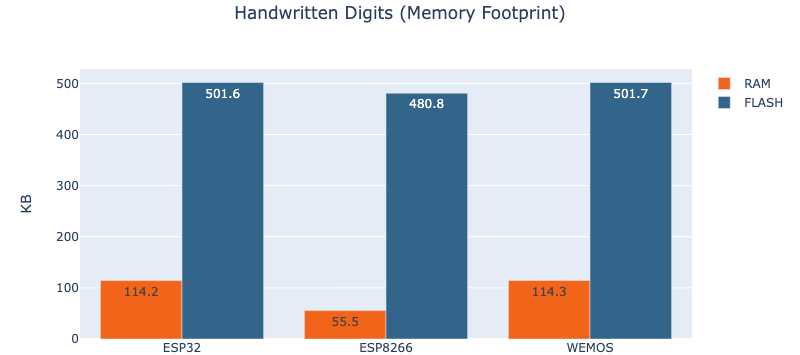
\includegraphics[width=0.6\textwidth]{HD-Mem-KB.png}
    \caption{HD Memory Footprint KB.}
    \label{fig:12}
\end{figure}

Figure \ref{fig:12} shows the memory usage (in KB) of the boards in relation to the Handwritten Digits model. The x-axis represents the type of microcontroller, while the y-axis represents the amount of memory in KB. ESP8266 occupies less FLASH memory in KB than the other two microcontrollers, while the RAM is about half compared to ESP32 and WEMOS. ESP32 and WEMOS are pretty much the same.

\begin{figure}[H]
    \centering
    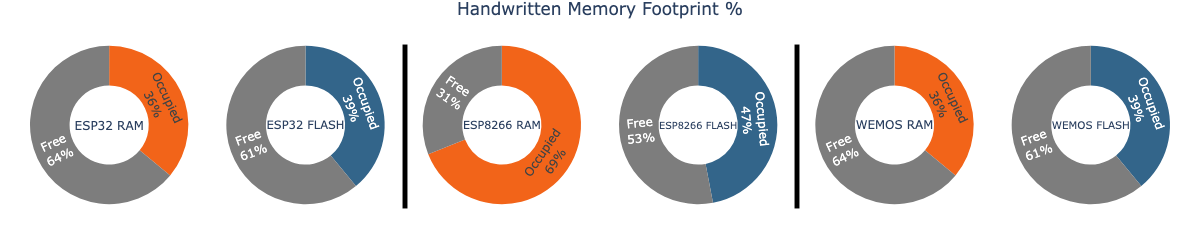
\includegraphics[width=1.0\textwidth]{HD-Mem-perc.png}
    \caption{HD Memory Footprint Percentages.}
    \label{fig:13}
\end{figure}

Figure \ref{fig:13} shows the memory usage as a percentage in relation to the Handwritten Digits model of the three microcontrollers. ESP32 and WEMOS have the same percentage of occupied memory because the available memory is the same. The percentage of FLASH memory occupied by ESP8266 is a little higher than ESP32 and WEMOS, while the RAM is much higher.

\subsection{AQ Memory Footprint}

\begin{figure}[H]
    \centering
    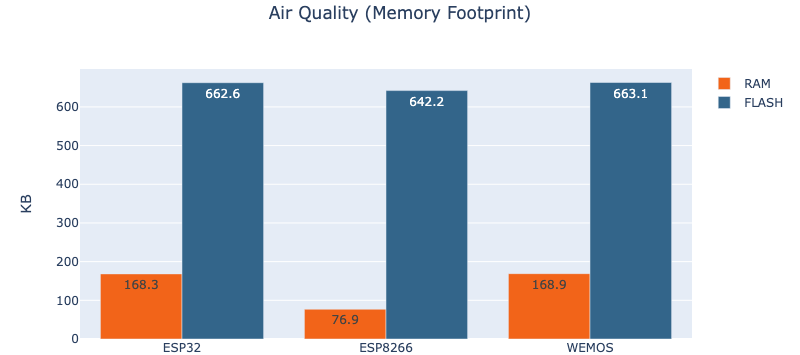
\includegraphics[width=0.6\textwidth]{AQ-Mem-KB.png}
    \caption{AQ Memory Footprint KB.}
    \label{fig:14}
\end{figure}

Figure \ref{fig:14} shows the memory usage in KB of the three microcontrollers using the Air Quality model. The x-axis represents the type of boards, while the y-axis represents the amount of memory in KB. The ESP32 and WEMOS have a similar memory footprint for both RAM and FLASH memory types. The used memory of the ESP8266 is similar for FLASH and much lower for RAM compared to ESP32 and WEMOS.

\begin{figure}[H]
    \centering
    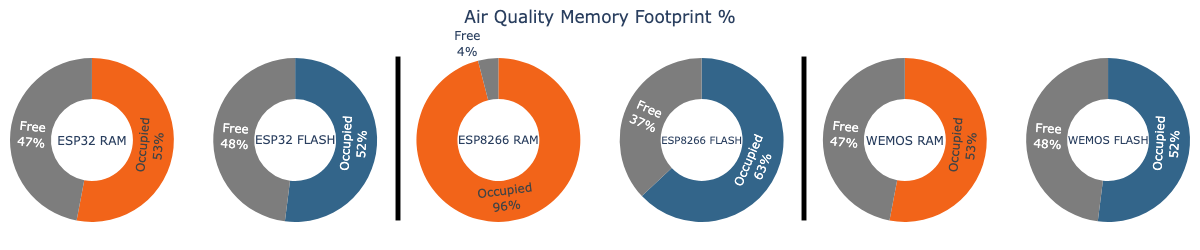
\includegraphics[width=1.0\textwidth]{AQ-Mem-perc.png}
    \caption{AQ Memory Footprint Percentages.}
    \label{fig:15}
\end{figure}

Figure \ref{fig:15} shows the percentage of memory used by ESP32, ESP8266 and WEMOS using the Air Quality model. The percentage of memory used by ESP32 and WEMOS is exactly the same because the available memory is the same. In this case the Air Quality model on the ESP8266 occupies 96\% of the RAM memory. This means that the ESP8266 operation is very limited, the memory is almost full.

\subsection{FC Memory Footprint}

\begin{figure}[H]
    \centering
    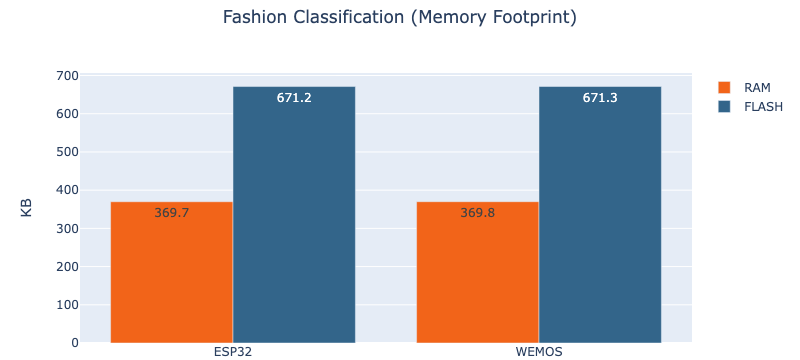
\includegraphics[width=0.6\textwidth]{FC-Mem-KB.png}
    \caption{FC Memory Footprint KB.}
    \label{fig:16}
\end{figure}

Figure \ref{fig:16} shows the memory usage in KB of the ESP32 and WEMOS using the Fashion Classification model. The x-axis represents the type of boards, while the y-axis represents the amount of memory in KB. The ESP8266 board was unable to run this model due to insufficient RAM space. Therefore, the performance of this model on the ESP8266 board will not be considered. The memory occupied by ESP32 and WEMOS turns out to be exactly the same.

\begin{figure}[H]
    \centering
    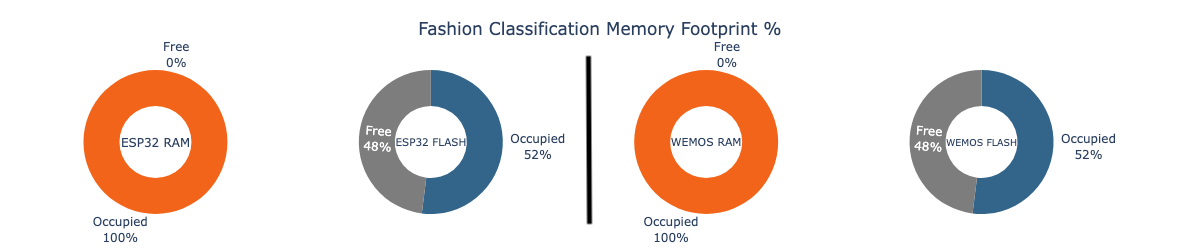
\includegraphics[width=1.0\textwidth]{FC-Mem-perc.png}
    \caption{FC Memory Footprint Percentages.}
    \label{fig:17}
\end{figure}

Figure \ref{fig:17} shows the percentage of memory used by ESP32 and WEMOS using the Fashion Classification model. ESP32 and WEMOS have the same percentage of occupied memory.

\section{Conclusion}

The ESP8266 board has higher prediction times and higher memory consumption (as a percentage) than the other two microcontrollers. Prediction times turn out to be very distant from ESP32 and WEMOS, in fact the prediction performance of the ESP8266 does not come close when running all ML models. 

Regarding ESP32 and WEMOS it can be said that their performance is very close to each other. In fact, the memory consumption during the execution of all models considered it's pretty much the same. However, the main difference between the two microcontrollers is the speed of model prediction. In fact, the prediction speed of WEMOS turns out to be faster than that of ESP32, even if the difference is not much.

It is therefore possible to conclude that WEMOS is the most performing microcontroller among those analysed.

\end{document}
